%# -*- coding: utf-8-unix -*-
% !TEX program = xelatex
% !TEX root = ../thesis.tex
% !TEX encoding = UTF-8 Unicode
%%==================================================
%% chapter01.tex for SJTU Master Thesis
%%==================================================

%\bibliographystyle{sjtu2}%[此处用于每章都生产参考文献]
\chapter{Introduction}
\label{chap:intro}
\section{Introduction}
People have their own opinions, and sometimes they change their opinions in response to others that hold views on given issues. Their opinions are reflected to the leader to make laws and vital decision. These phenomena can be found out  in some cases, such as voting, legislation and adoption of new policies. It is widely recognized that opinion formation and decision making formation have mutual interaction as interconnected networks.\parencite{mikko2014, danziger2019, newman2010, boccaletti2014, domenico2013, tomasini2015, namkhanhvu2017}. And sometimes, opinion formation could be opposed to decision making formation. These situations often make social conflict and cause social confusion. To figure out these social conflicts, it is needed to understand and analyze the competition of interconnected networks. So far, physics and computer science have researched these social conflict by modeling and analyzing the complex systems\parencite{fangwu2004, zuev2012, laguna2004, masuda2014}. The researches include opinion dynamics, voter model, game theory and many more.\parencite{smyrnakis2019, bianconi2018, redner2017, haibo2017, amato2017, quattrociocchi2014, casey2009} 
Competition of interconnected networks has been researched in many ways. These networks can be applied to the dissemination of computer viruses, messages, opinions, memes, diseases and rumors\parencite{hua2014,shenyu2018, zhou2018, alvarez2016,gomez2015,diep2017,rocca2014,velasquez2018}. Opinion dynamics on interconnected networks has been investigated with various network models such as \textit{Abrams-Strogatz(AS)} model\parencite{abrams2003,vazquez2010} and $M$ model\parencite{rocca2014}.  Based on the previous researches, we would study the main features of competing two-layer networks by changing network structures, changing the time-related updating rules to interact on two-layers, and finding the key nodes on layers. The simulation results of changing network structures presents how the network structures, which include internal degrees, external degrees and network type, affect the state of network. Changing the way to interact on two-layers are related to updating rules, and it would be proven that different updating rules cause different results. In addition, it would be analyzed that what updating rules mean in real world. Last, finding key nodes show that which node centrality is the most influential to change network state on the interconnected network. 
\begin{figure}[!htb]
	\centering
	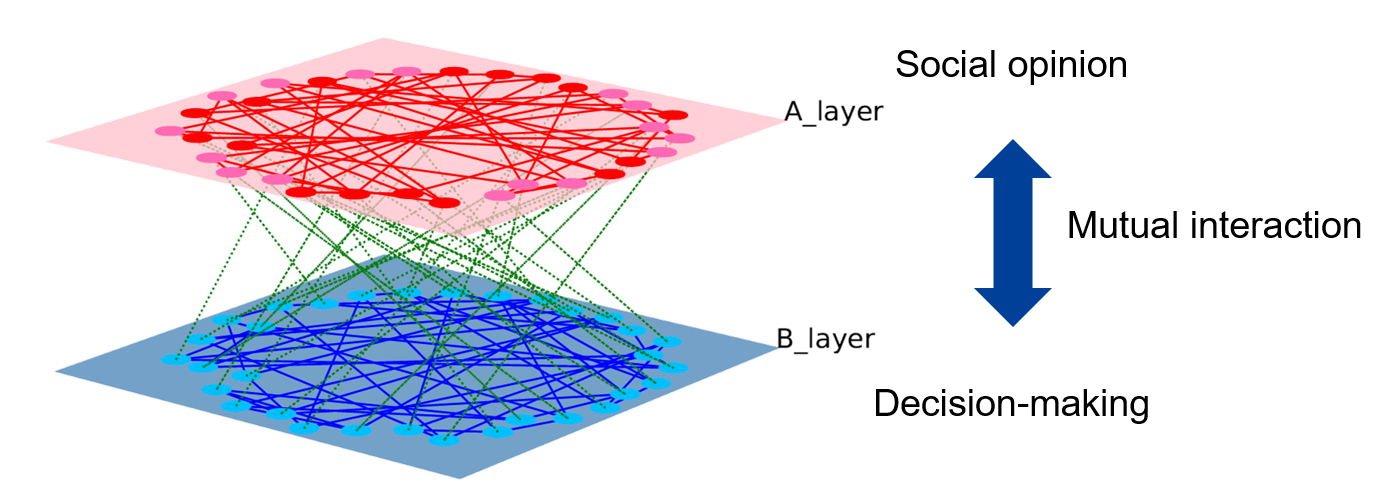
\includegraphics[width=\hsize]{chap1_topic.png}
	\caption{The example of competition on two-layer network}
	\label{chap1_topic}
\end{figure}

\section{Related Work}
In this research, we focus on the competition on two layer network or interconnected network. Comparing with single layer, interconnected network has 2 dynamics, 2 parameters and include internal edge and external edge as shown in Fig.~\ref{chap1_singlemulti}. Therefore, multi-layer network interaction would be more complex than single layer network interaction.
\begin{figure}[!htb]
	\centering
	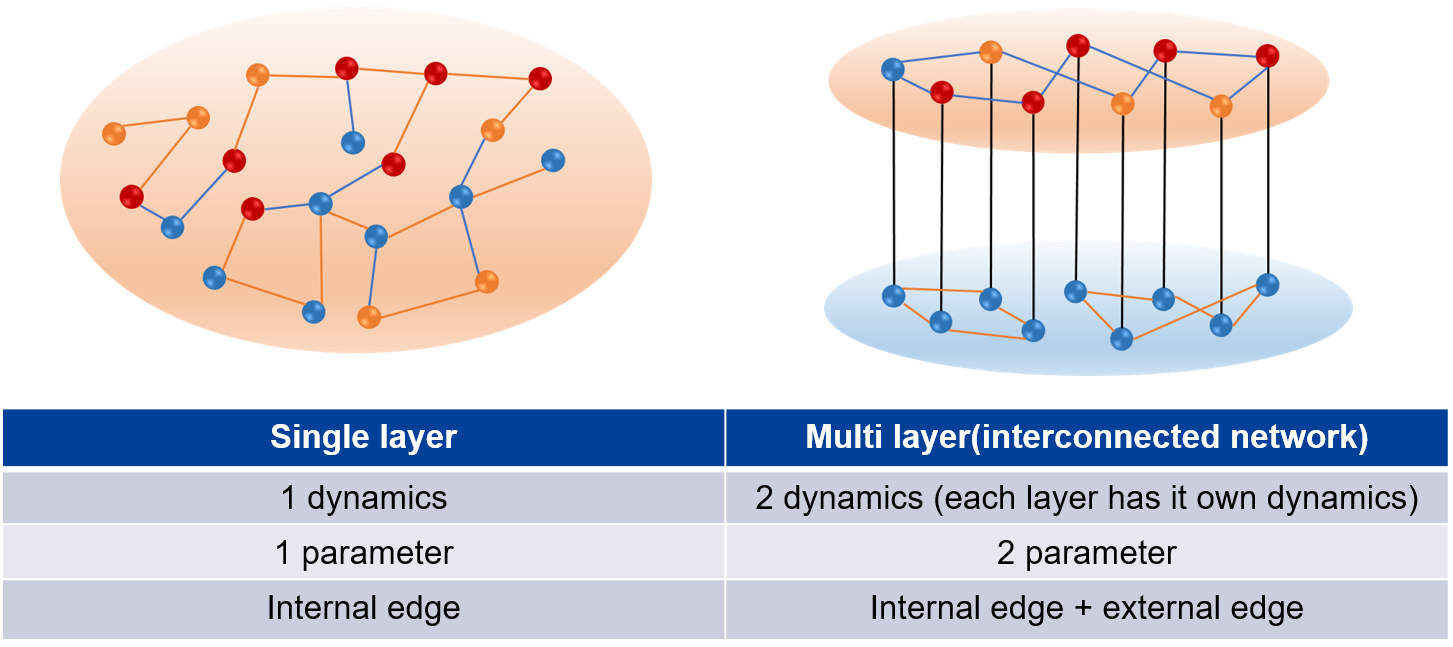
\includegraphics[width=\hsize]{chap1_singlemulti.png}
	\caption{Comparison between single layer and multi-layer}
	\label{chap1_singlemulti}
\end{figure}
To make two layer networks under competition, each layer is made up with different dynamics and parameter. Network dynamics are based on previous research such as \parencite{alvarez2016}. One layer has the function of social opinion and its own dynamics. Some opinion models provide social mechanism by means of a compromise process.\parencite{naim2003} Other opinion models represent persuasive process.\parencite{chau2014} In this paper, the social opinion layer is affected by the opinion dynamics which are also known as M-model\parencite{rocca2014}, that includes compromise function and persuasion function. The other layer also has the function of decision-making and its own dynamics. The dynamics of the decision making layer is the language competition dynamics that are also called as Abrams-Strogatz model\parencite{abrams2003, vazquez2010, patriarca2012}. This model is useful to decide only one opinion from two opinions. For competition condition, the initial status of the two layers is assumed to be in opposite states, that social opinion layer has all positive states and decision making layer has all negative states.
So far, main researches have focused on what factors make a consensus or dissent, which have shown that the system can make positive consensus, negative consensus or coexistence under certain range of parameters, such as volatility, reinforcement and prestige.\parencite{alvarez2016} And interconnected competition of the social network have been researched by finding the threshold or critical point for consensus.\parencite{alvarez2016, gomez2015, diep2017}
Also, it has been found out that the thresholds make the transition of states and they can explain and analyze the social phenomena in real world such as the legislation, election and social conflicts.\parencite{alvarez2016, amato2017, diep2017} In \parencite{gomez2015}, it is shown that the transition from localized to mixed status occurs through a cascade from poorly connected nodes in the layers to the highly connected ones and the number of external degree is very important to change the state of layers.\parencite{gomez2015} In addition, the main features, such as transition and cascade, found in Monte Carlo simulation are exactly characterized by the mean-field theory and magnetization\parencite{alvarez2016, diep2017, amato2017, gomez2015}. 
Based on these pre-existed researches, the competition of interconnected network would be analyzed by 3 main topics, such as network structures, updating rules and node centralities. Prior to simulations, backgrounds for 3 topics would be explained as follows. 
\begin{figure}[!htb]
	\centering
	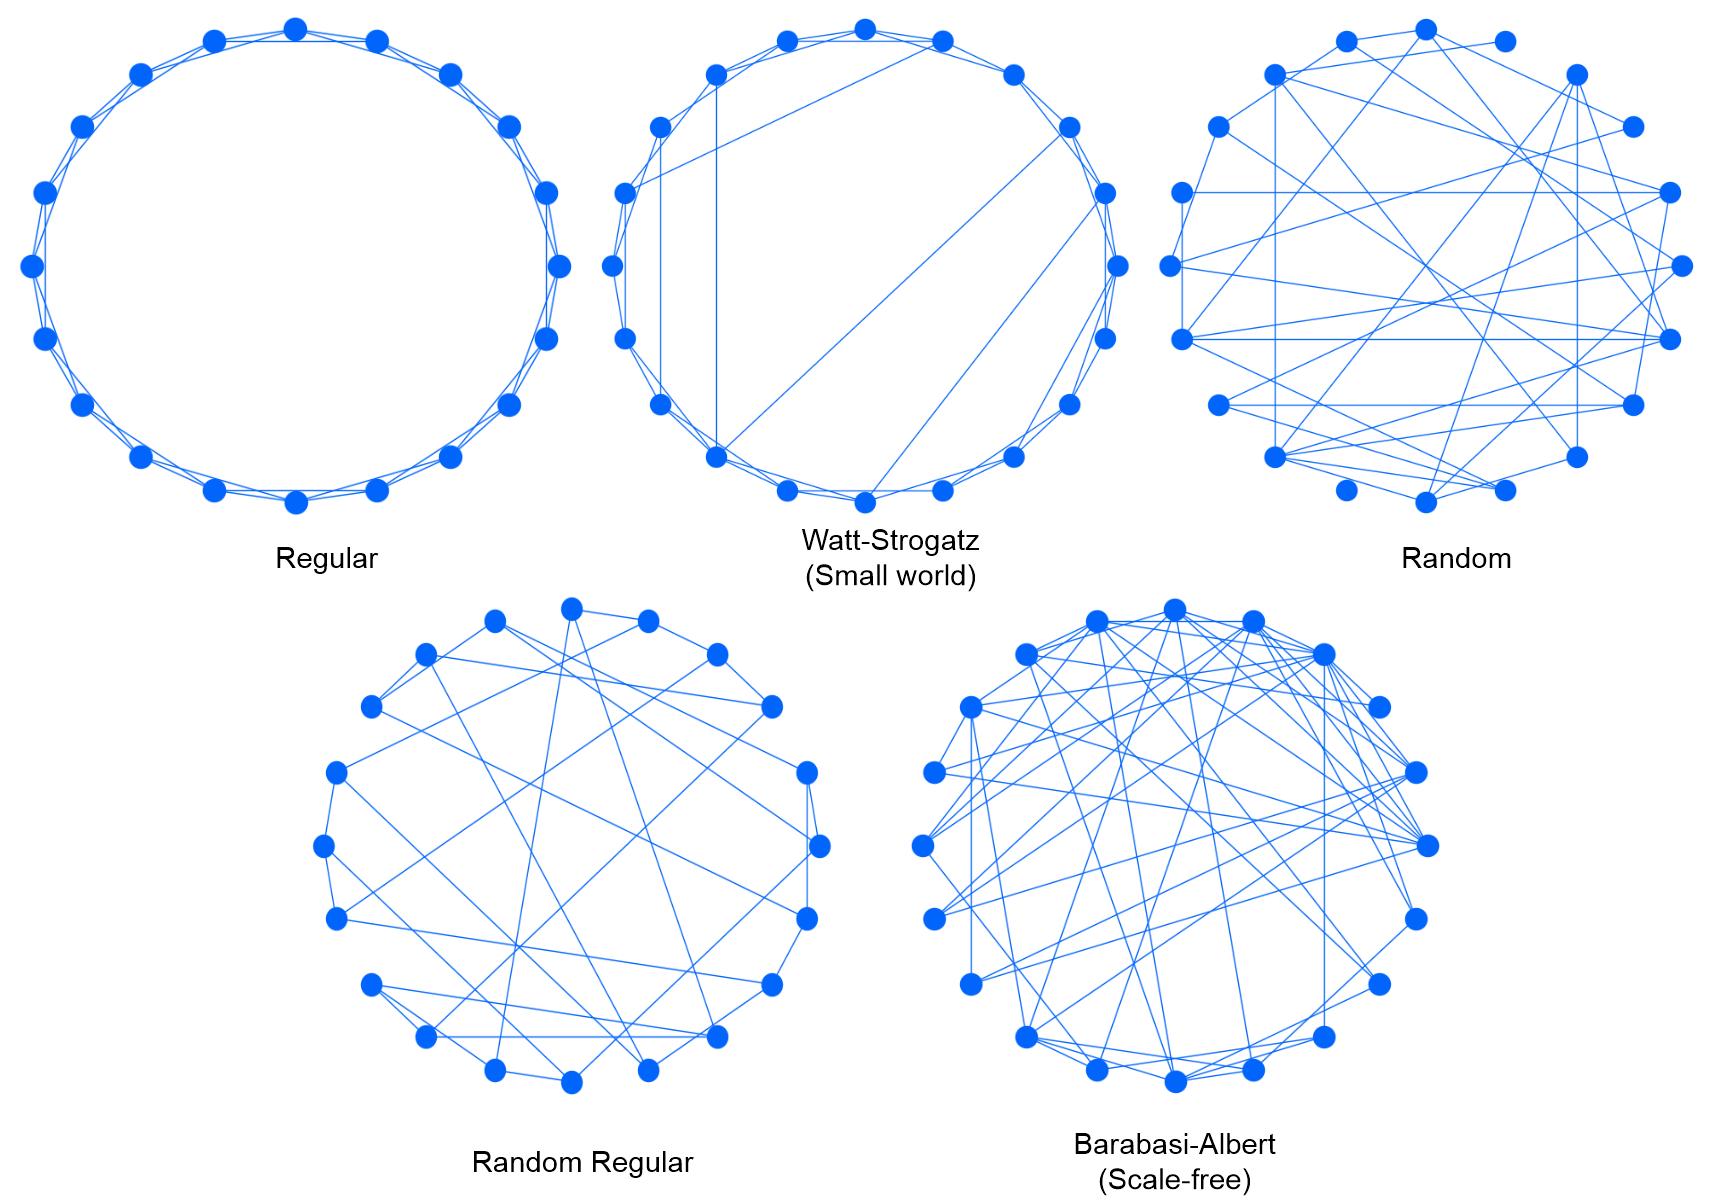
\includegraphics[width=\hsize]{chap1_network_type.png}
	\caption{Various structures of network}
	\label{chap1_network_type}
\end{figure}
First, network structures would be investigated to change the structure of network. Networks could be largely divided into regular network, random network\parencite{erdos1960}, small world network\parencite{watts1998}, scale free network\parencite{barabasi1999} and others. Fig.~\ref{chap1_network_type} shows the graph of various networks. 
Regular network has lattice structure, and  each node has exactly the same number of links. Random network is made up with edges that two node are connected with probability $p$ in the systems with $K$ nodes. 
Small world network is a network graph in which most nodes are not neighbors of one another, but most nodes can be reached from every other node by a small number of links. Small world network can be made by eliminating the edges with probability $p$ and connecting two random nodes that are not connected in a regular network. Small world network has all characteristics of regular network and random network.
Scale free network has the model that distribution of edges follows power function. Examples of scale free network are the World Wide Web (WWW), the Internet, movie star networks, protein interactions, metabolism, and so on.
There are several ways to create a scale free network. Among them, the most typical way is Barabasi-Albert models.
The \textit{Barabasi-Albert} model is growing networks in which nodes continue to be added, and connections between nodes has preferential attachment. The process of creating this model repeats the following two processes: First, add one node with a constant number of edges to the system. Second, edges of the added nodes are connected in proportion to edges number of the pre-existing nodes.
In this paper, two type of general network would be applied such as random regular(RR) network and \textit{Barabasi-Albert}(BA) network. 

Second, dynamics orders and time-related updating rules would be studied. For further understanding the competition on two layer network, it is very important to investigate the interaction between nodes or layers. Methods of interaction between nodes are very various.\parencite{sirbu2017} But, related to time, the types of interactions  would be divided into two categories, simultaneous interaction and sequential interaction. In economics and social networks, it has been proven that there exists different results between simultaneous and sequential interactions.\parencite{hoffman2011, dietrich2004} In \parencite{hoffman2011}, it was researched that how experimental subjects update induced prior information when receiving two information signals simultaneously or receiving the same signals sequentially. As the experimental results, the simultaneous treatment is very different from sequential treatment, and under sequential information,  subjects’ mean estimates of the two treatments(good news preceding bad news or vice versa) are also significantly different from each other. In conclusion, both sequencing and the order of information processing suggest which one arrives matters. And, in \parencite{dietrich2004}, the usual random sequential updating rule is replaced  by simultaneous updating on the Sznajd model. As the results, it is found out that this change makes a complete consensus much more difficult. The reason is analyzed as that for simultaneous updating some agents simultaneously receive conflicting messages from different neighbor pairs and thus refuse to change their opinion. In this paper, both simultaneous and sequential updating rules would be applied to layers, nodes and links. 

Third, network centralities would be researched to find key nodes on two layers network. Network centrality means the index to measure how close each node is to the center of the network. Than means answers to the question "What characterizes an important node?". The concept of network centrality was first introduced in the field of social network analysis.\parencite{freeman1979} After that, it has expanded to various areas where the concept of the network is related and has been used to identify which nodes are important in the network. So far, various criteria for assessing network centrality have been presented. Generally well-known network centralities include degree centrality, betweeness centrality, closeness centrality, eigenvector centrality and pagerank centrality.\parencite{koschutzki2008}
Degree centrality is the simplest but the most reliable concept. it is defined as the number of interacting neighbor nodes (or edges). Betweenness centrality is the concept of using the shortest path between two nodes on a network. It is explained as the concept to  define two different node sets on the network (set 1, 2) and quantify how often each node appears on the shortest path for all combinations of nodes in set 1 and set 2. Closeness centrality is derived from that the shorter the path that one node reaches all the other nodes is, the more important the node is. Eigenvector centrality is the concept that the more a node is connected with critical nodes, the more important it is. Pagerank centrality measures the convergent value by repeating the process of propagating each node's influence to the other nodes. 
So far, many researchers have been trying to find important nodes in social network.\parencite{eom2015, white2003, mesgari2015, hwang1981, huang2014} Based on node centrality, some algorithms for identifying key nodes has been found out. In \parencite{mesgari2015, huang2014}, it has been found out that optimally combining multiple measures of nodal importance may provide a robust tool for identifying key nodes of interest, particularly in large graphs. Here, based on previous research, we would try to find the key nodes by using single node centrality and combined node centrality. 

In this paper, as the single indicator methods to find key nodes, network centralities would be applied such as pagerank, degree centrality, eigenvector centrality, betweenness and closeness.\parencite{francisco2019, bianconi2018}. As the multiple indicator methods to recognize key nodes, several combined node centralities would be applied such as \textit{PR+DE, PR+BE, DE+BE, PR+DE+BE} that are based on single indicators.  By using these centralities(pagerank, degree, eigenvector, closeness, betweenness and combined node centralities), it would be found out that which method is the most influential to change the network states on various models.  

\section{Thesis Objective and Direction}
In this paper, opinion dynamics of a competing two-layer social network are investigated on the basis of the pre-existed research\parencite{alvarez2016, gomez2015, diep2017, rocca2014}. We develop the previous modeling and research to find out the characteristics of interconnected networks. By switching the network structure and updating rule of each layer, we can see how the consensus or coexistence states change and what conditions make the social consensus or dissent. In addition, trying to identifying key nodes on various network structures, it would be found out which method works well.  

This Research has 4 main directions. First, it would be provided how to make up competition models and how to measure the consensus for analysis. Second, it would be found out what factors make consensus by changing network structures. Third, it would be analyzed how dynamics orders and time-related updating rules have an influence on status of two-layer. Fourth, it would be investigated which method is the most effective to identify key nodes based on node centralities. These study can help to explain social networks phenomena, such as social conflict between social opinion and the congress. Therefore, this research could be used as a tool for analyzing legislation problems, making efficient decision-making system and solving the social conflict. 

This paper is organized as follows. In chapter 2, it is introduced that how competing two layers are made up and how the dynamics of each layer works. And some indexes are provided to measure and evaluate the simulation results. In chapter 3, with changing network structure, it would be found out that how the network structures have the influence on the consensus of two layers. In chapter 4, considering the dynamics orders and time-related updating rules, simulation results would be compared and analyzed. In chapter 5, it would be researched that which nodes are important to affect the state of network by using single indicators and multiple indicators. Finally, in chapter 6, all simulation results will be summarized and our findings are concluded. And it is considered that what would be researched as future works and how we can be applied to real world. 


